\chapter{Introducción}
\label{ch:intro}

\section{Descripción del problema}
\label{sec:DescripcionProblema}
El objetivo de este trabajo es el desarrollo de una planta 
educativa de control de nivel
(\textit{Level control trainer}).
La planta será utilizada para realizar prácticas con los
alumnos, perimitiendo aplicar los conceptos de 
control de procesos, programación de \gls{plc}, SCADA,
Ajuste de lazos PID, Teoría de Cascadas. 
Además, el alumno tendrá la aproximación a elementos de adquisición que 
se encuentran en la industria, tales como sensores diferenciales de presión
(\textit{DP cell}) y placas orificio.
El proyecto está destinado a ser utilizado por las cátedras de
Automatismos Industriales, Autómatas y Control Discreto 
(Ingeniería en Mecatrónica)
como así también Instrumentación y Control Automático (Ingeniería Industrial
y de Petróleos)\todo{verificar}.

En la actualidad, en el Laboratorio de Control Automático de la Facultad, 
se disponen con equipos similares al descripto\todo{citar equipos?}.
No obstante, el proyecto planteado tiene la característica de ser 
\textbf{móvil}: se encuentra montado en una estructura que 
permite su desplazamiento, y el enlace a la 
computadora de control se realizará de manera inalámbrica.
% Además, se utilizará una válvula neumática...

Se encuentran en el mercado plantas similares, llave en mano. 
Dos firmas del medio fueron consultadas, para conocer 
el precio en el mercado de un desarrollo similar:
\begin{itemize}
 \item \textbf{Reino Unido}: Una planta con características similares
 a la descripta tiene un precio de $16225\,USD$ en puerto de Buenos Aires
 \item \textbf{Italia}: Con un precio de $28403\,EUR$ en puerto. 
 El modelo propuesto por la firma italiana
 posee un precio superior debido a que está construído en acero inoxidable.
\end{itemize}

Se observa que, debido al elevado costo del producto en el mercado,
se justifica su desarrollo  y construcción en la facultad.
Se plantea entonces el desafío de diseñar, ensamblar y programar una planta
móvil de control de nivel en el Laboratorio de Control Automático de la Facultad.

%Por qué se hizo el trabajo? Comparación con otras plantas
%(plantas para comprar Y plantas que puglesi ya tiene)

\subsection{Especificaciones}

Las siguientes especificaciones deben cumplirse para la nueva
planta:

\begin{itemize}
\item Debe cumplir su objetivo pedagógico, permitiendo 
 a los alumnos comprender los principios del control automático.
 \item Su costo debe ser inferior a una solución llave en mano.
 \item Deberán utilizarse actuadores, elementos de adquisición
 y controladores que se encuentren en plantas industriales.
 \item Representación de fenomenos que afectan los procesos 
 industriales, tales como perturbaciones en bombas y tiempo 
 muerto en los procesos. 
 \item Se confeccionará un manual de uso sencillo, para 
 fácil comprensión por parte de los alumnos.

\end{itemize}
\todo{Mejorar}

\section{Materiales disponibles}
\label{sec:MaterialesDisponibles}

A la hora de comenzar con el proyecto, varios elementos habían
sido adquiridos por el director de proyecto y se encontraban
disponibles en el Laboratorio de Control Automático:
\begin{itemize}
 \item \textbf{Válvula neumática:} marca Foxboro, modelo Stabilflo (serie V1), para controlar el 
 caudal. Se trata de una válvula isoporcentual, con un electroposicionador Power Genex.
 La apertura de la válvula será nuestra variable de control en el sistema. 
 Ver sección \ref{sec:ValvulaNeumatica}.
  \item \textbf{Electrobombas monofásicas (2):} impulsarán el fluido
  en la planta de control de nivel.
  La velocidad de las bombas (frecuencia) no será controlada.
  Ver sección \ref{sec:Bombas}.
  \item \textbf{Placa Orificio:} Permite estimar el 
  caudal en un tubo midiendo la presión.
  Se tratará en la sección \ref{subsec:PlacaOrificio}.
  \item \textbf{DP cells (2):} Sensores de presión 
  diferencial marca Yokogawa. 
  Uno de los sensores será utilizado para medir el nivel del tanque controlado,
  en tanto que el segundo medirá caudal con la ayuda de la placa orificio.
  Ver sección \ref{subsec:DPCell}.
  \item \textbf{Instrumentos de protección y comando:}
  Para las bombas, podemos citar: Contactores, relés, 
  Llaves termomagnéticas\todo{verificar}.
  Ver sección \ref{sec:Potencia}.
  \item{\textbf{\gls{plc}}}: Twido 40 DTK (Siemens) con un módulo
  analógico TWDAMM6HT y su correspondiente fuente de alimentación.
  Permitirá controlar las bombas (encendido/apagado), 
  leer valores de presión de las DP Cell y modificar la apertura de la 
  válvula. Ver sección \ref{subsec:plc}.
  \item \textbf{Estructura:} un marco móvil, montado sobre ruedas,
  se encuentra disponible. Ver Sección \ref{sec:EstructuraSoporte}.
  \item \textbf{Cañerías y accesorios}: Serán utilizados para 
  conectar los elementos de la planta. Ver sección \ref{sec:Canerias}.
  \item \textbf{Manómetros (2):} A colocar en 
  puntos específicos de la planta.
  \item \textbf{Módulos inalámbricos:} Marca CTM Electrónica,
  modelo AD-xxx\todo{Verificar modelo}, permite enlazar la 
  interfaz RS485 a la computadora de control
  de manera inalámbrica. Ver sección \ref{subsec:inalambrico}.
\end{itemize}

A partir de los materias disponibles, se confeccionó 
un proyecto de planta, estableciendo las tareas a realizar, el orden
y un planning de trabajo.

\section{Solución propuesta}
\label{sec:SolucionPropuesta}

Mediante los materiales disponibles se dispone a la construcción de 
una planta de control de nivel. En esta, dos tanques son alimentados por 
dos bombas de acción reciproca y mediante una válvula neumática se actuá
sobre el sistema para su control. El nivel del tanque controlado es medido 
mediante celdas de presión diferencial.

Para poder recrear fenómenos que afectan los procesos industriales se agregan
a la planta:
\begin{itemize}
\item X\todo{Cuantos metros} metros de cañería que sirven como tiempo muerto
de la planta.
\item La conexión, mediante una válvula manual, de la salida con la entrada
 de la bomba de manera de simular las perturbaciones del circuito hidráulico.
\end{itemize}

Resulta de interés la implementación de Teoría de Cascadas y para ello se pone
a disposición en la planta la medición del caudal circulante mediante un elemento
depresor\todo{Placa Orificio} y una celda de presión diferencial.

\section{Organización}
\label{sec:Organizacion}
\subsection{División del trabajo}
Dado que la construcción de la planta implica una serie de etapas que
deben realizarse de manera seriada, se dividió el trabajo en los siguientes puntos:
\begin{enumerate}
 \item \textbf{Planificación y diseño preliminar}:
  \item \textbf{Construcción de la planta}
  \begin{enumerate}
   \item Preparación de la estructura
   \item Montaje de los elementos de la planta
   \item Cañerías
   \item Cableado eléctrico de potencia
   \item Cableado de señal: PLC, válvula, DP cells, módulo inalámbrico.
   \item Pruebas de funcionamiento sencillo
   \item Pintura y acabados
  \end{enumerate}
  \item \textbf{Programación del \gls{plc}}
  \item \textbf{Programación del software SCADA}
  \item \textbf{Pruebas de funcionamiento}
  \item \textbf{Documentación}
\end{enumerate}

\subsection{Planning}
\begin{figure}[ht!]
	\centering
	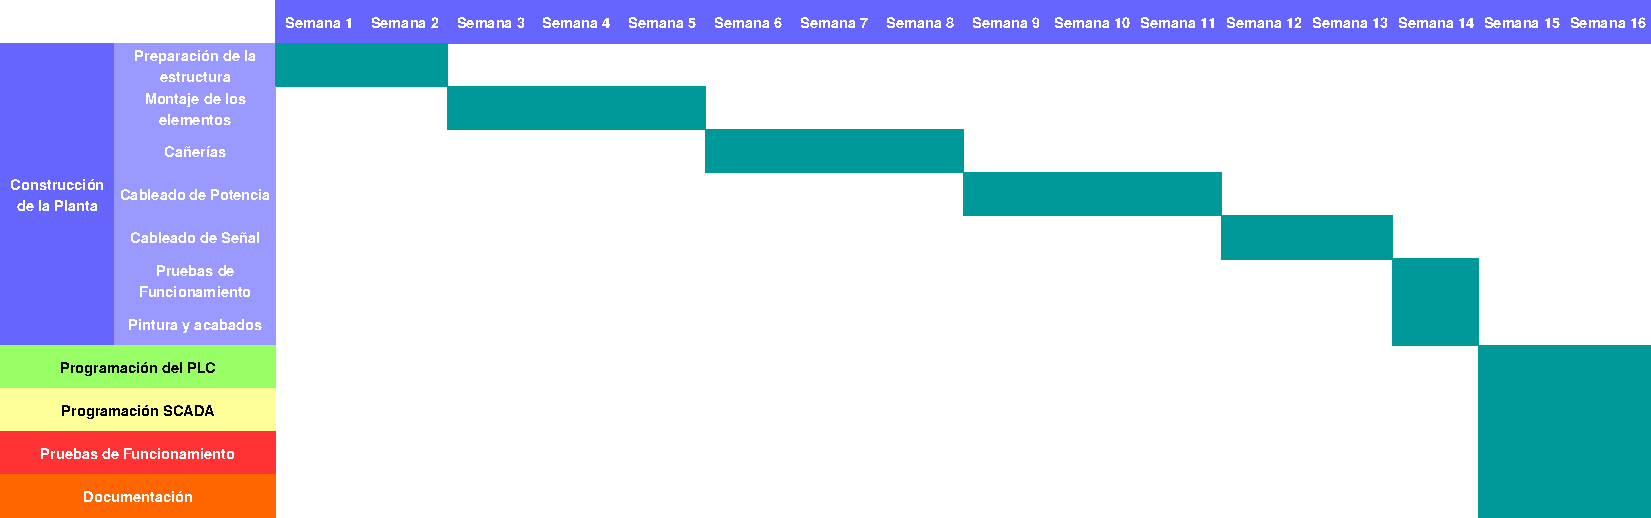
\includegraphics[angle=-90,width=0.44\textwidth]{Cap1-Introduccion/images/EDT.pdf}%width=.9\textwidth
	\caption{Esquema de la division del tiempo}
	\label{fig:EDT}
\end{figure}
